% Preamble
\documentclass[12pt, twoside]{book}
\usepackage[utf8]{inputenc}
\usepackage{graphicx}
\usepackage{amsmath}
\usepackage{amsfonts}
\usepackage{nicematrix}
\usepackage{algorithm}
\usepackage{algpseudocode}
\usepackage{mathtools} % dcases
\usepackage{multicol}
\usepackage{tcolorbox}
\usepackage{datetime}
\usepackage{caption}
\usepackage{etoolbox}
\usepackage{subfig}
\usepackage{algcompatible}
\usepackage{algpseudocode}
\usepackage{setspace}
\usepackage[a4paper,left=40mm,right=20mm,top=20mm,bottom=20mm,bindingoffset=0mm]{geometry}
\usepackage{fancyhdr}
\usepackage{listings}
\usepackage{color}
\usepackage{hyperref}
\usepackage{enumitem}
\usepackage[acronym]{glossaries}

% Telugu script
\usepackage{fontspec}
\newfontfamily{\tel}[Script=Telugu]{Mandali}

% Custom colors
\definecolor{deepblue}{rgb}{0,0,0.5}
\definecolor{deepred}{rgb}{0.6,0,0}
\definecolor{deepgreen}{rgb}{0,0.5,0}

% Python style for highlighting

\newtheorem{theorem}{Theorem}[section]
\newtheorem{definition}{Definition}[section]
\newtheorem{notation}{Notation}[section]
\newtheorem{remark}{Remark}[section]
\newtheorem{corollary}{Corollary}[theorem]
\newtheorem{lemma}[theorem]{Lemma}
\newtheorem{problem}[theorem]{Problem}

\newcommand{\twopartdef}[4]
{
	\left\{
		\begin{array}{ll}
			#1 & \mbox{if } #2 \\
			#3 & \mbox{if } #4
		\end{array}
	\right.
}

\AtBeginEnvironment{tcolorbox}{\footnotesize}

\newdateformat{monthyeardate}{%
  \monthname[\THEMONTH], \THEYEAR}

\graphicspath{ {images/} }

% \usepackage[a4paper,width=150mm,top=20mm,bottom=20mm,bindingoffset=6mm]{geometry}


\fancypagestyle{fancy}{
\fancyhead{}
% \fancyhead[RO,LE]{Modern Research Software For Fast Multipole Methods}
\fancyhead[RO,LE]{\nouppercase{\leftmark}} % Automatically use the chapter title
\fancyfoot{}
\fancyfoot[LE,RO]{\thepage}
}

\fancypagestyle{chaptertitle}{
  \fancyhf{} % Clear all header and footer fields
  \fancyfoot[LE,RO]{\thepage}
  \renewcommand{\headrulewidth}{0pt} % Remove header line
}

\fancypagestyle{plain}{
  \fancyhf{} % clear all header and footer fields
  \fancyfoot[C]{}
  \renewcommand{\headrulewidth}{0pt} % remove header line
  \renewcommand{\footrulewidth}{0pt} % remove footer line
\fancyfoot[LE,RO]{\thepage}
}

\usepackage{titlesec}

\titleformat{\chapter}[display]
  {\normalfont\bfseries}{}{0pt}{\Huge}

\usepackage[backend=bibtex]{biblatex}
\addbibresource{references.bib}

% Slightly cleaner tables
\usepackage{booktabs}

% Clear a page after current page is done
\usepackage{afterpage}

% Filler
\usepackage{lipsum}

% Shortcuts
\def\Htwo{\mathcal{H}^2}
\def\H{\mathcal{H}}
\def\R{\mathbb{R}}
\def\Rtwo{\mathbb{R}^2}
\def\Rthree{\mathbb{R}^3}
\def\Rd{\mathbb{R}^d}
\def\Xbf{\mathbf{x}}
\def\Ybf{\mathbf{y}}


% % Shortcuts
% \newtheorem{theorem}{Theorem}[section]
% \newtheorem{definition}{Definition}[section]
% \newtheorem{notation}{Notation}[section]
% \newtheorem{remark}{Remark}[section]
% \newtheorem{corollary}{Corollary}[theorem]
% \newtheorem{lemma}[theorem]{Lemma}
% \newtheorem{problem}[theorem]{Problem}

% Default fixed font does not support bold face
\DeclareFixedFont{\ttb}{T1}{txtt}{bx}{n}{12} % for bold
\DeclareFixedFont{\ttm}{T1}{txtt}{m}{n}{12}  % for normal

% Custom code colors
\usepackage{listings}
\usepackage{xcolor}

\lstset{basicstyle=\small\ttfamily}
\definecolor{codegreen}{rgb}{0,0.6,0}
\definecolor{codegray}{rgb}{0.5,0.5,0.5}
\definecolor{codepurple}{rgb}{0.58,0,0.82}
\definecolor{backcolour}{rgb}{0.95,0.95,0.92}

\lstdefinestyle{mystyle}{
    backgroundcolor=\color{backcolour},
    commentstyle=\color{codegreen},
    keywordstyle=\color{magenta},
    numberstyle=\tiny\color{codegray},
    stringstyle=\color{codepurple},
    basicstyle=\ttfamily\small,
    breakatwhitespace=false,
    breaklines=true,
    captionpos=b,
    keepspaces=true,
    numbers=left,
    numbersep=5pt,
    showspaces=false,
    showstringspaces=false,
    showtabs=false,
    tabsize=2
}

\lstset{style=mystyle}

% \definecolor{rustorange}{rgb}{0.8,0.4,0}
% \definecolor{codegray}{rgb}{0.5,0.5,0.5}
% \definecolor{backcolour}{rgb}{0.95,0.95,0.92}

% \lstdefinelanguage{Rust}{
%     keywords={type, as, break, const, continue, crate, else, enum, extern, false, fn, for, if, impl, in, let, loop, match, mod, move, mut, pub, ref, return, Self, self, static, struct, super, trait, true, type, unsafe, use, where, while, async, await, dyn},
%     keywordstyle=\color{rustorange},
%     commentstyle=\color{codegray},
%     stringstyle=\color{codepurple},
%     basicstyle=\ttfamily\small,
%     breakatwhitespace=false,
%     breaklines=true,
%     captionpos=b,
%     keepspaces=true,
%     numbers=left,
%     numbersep=5pt,
%     showspaces=false,
%     showstringspaces=false,
%     showtabs=false,
%     tabsize=2,
%     morecomment=[l][\color{magenta}]{\#},
%     morestring=[b]',
%     morestring=[b]"
%     morecomment=[l]{//},
%     morecomment=[s]{/*}{*/},
%     stringstyle=\color{red},
%     sensitive=true
% }

\lstdefinelanguage{Rust}{
    keywords={fn, let, mut, match, trait, impl, extern, crate, mod, pub, ref, Self, self, super, use},
    keywordstyle=\color{blue},
    morecomment=[l]{//},
    morecomment=[s]{/*}{*/},
    morestring=[b]",
    stringstyle=\color{red},
    sensitive=true
}

\lstset{
    language=Rust,
    basicstyle=\ttfamily,
    commentstyle=\color{gray}
}

\lstset{backgroundcolor=\color{backcolour}, style=mystyle}

% Remove excess double page
\let\cleardoublepage\clearpage

\makeglossaries                    % Initialize glossaries
\newacronym[plural=CPUs, longplural=Central Processing Units]{cpu}{CPU}{Central Processing Unit}
\newacronym[plural=GPUs, longplural=Graphics Processing Units]{gpu}{GPU}{Graphics Processing Unit}
\newacronym[plural=ASICs, longplural=Application-Specific Integrated Circuit]{asic}{ASIC}{Application-Specific Integrated Circuit}
\newacronym{ram}{RAM}{Random Access Memory}
\newacronym[plural=flops, longplural=Floating Point Operations]{flop}{FLOP}{Floating Point Operation}
\newacronym{hpc}{HPC}{High Performance Computing}

\newacronym{sisd}{SISD}{Single Instruction Single Data}
\newacronym{simd}{SIMD}{Single Instruction Multiple Data}
\newacronym{mimd}{MIMD}{Multiple Instruction Multiple Data}
\newacronym{simt}{SIMT}{Single Instruction Multiple Threads}

\newacronym{ilp}{ILP}{Instruction Level Parallelism}
\newacronym{tlp}{TLP}{Thread Level Parallelism}
\newacronym{dlp}{DLP}{Data Level Parallelism}
\newacronym{clp}{CLP}{Core Level Parallelism}

\newacronym{neon}{Neon}{Arm SIMD Extensions}
\newacronym{sse}{SSE}{Streaming SIMD Extensions}
\newacronym{avx}{AVX}{Advanced Vector Extensions/Gesher New Instructions}
\newacronym{avx2}{AVX2}{Advanced Vector Extensions/Haswell New Instructions}
\newacronym{avx512}{AVX-512}{Advanced Vector Extensions 512 bit}


\newacronym{blas}{BLAS}{Basic Linear Algebra Subprograms}
\newacronym{l2l}{L2L}{Local to Local}
\newacronym{l2p}{L2P}{Local to Particle}
\newacronym{m2l}{M2L}{Multipole to Local}
\newacronym{m2p}{M2L}{Multipole to Particle}
\newacronym{m2m}{M2M}{Multipole to Multipole}
\newacronym{p2p}{P2P}{Particle to Particle}
\newacronym{p2m}{P2M}{Particle to Multipole}

\newacronym[plural=kiFMMs, longplural=kernel independent Fast Multipole Methods]{kifmm}{kiFMM}{kernel independent Fast Multipole Method}
\newacronym[plural=FMMs, longplural=Fast Multipole Methods]{fmm}{FMM}{Fast Multipole Method}
\newacronym[plural=PDEs]{pde}{PDE}{Partial Differential Equation}
\newacronym{mfs}{MFS}{Method of Fundamental Solutions}
\newacronym[plural=BIEs, longplural=Boundary Integral Equations]{bie}{BIE}{Boundary Integral Equation}
\newacronym[plural=BEMs, longplural=Boundary Element Methods]{bem}{BEM}{Boundary Element Method}
\newacronym[plural=FFTs, longplural=Fast Fourier Transforms]{fft}{FFT}{Fast Fourier Transform}

\doublespacing

\begin{document}



% declaration of the new block
\algblock{PARFOR}{ENDPARFOR}
% customising the new block
\algnewcommand\algorithmicparfor{\textbf{parfor}}
\algnewcommand\algorithmicpardo{\textbf{do}}
\algnewcommand\algorithmicendparfor{\textbf{end\ parfor}}
\algrenewtext{PARFOR}[1]{\algorithmicparfor\ #1\ \algorithmicpardo}
\algrenewtext{ENDPARFOR}{\algorithmicendparfor}

    \frontmatter
    \pagestyle{plain}

    \begin{titlepage}
    \begin{center}
        \vspace*{1cm}

        \Huge
        \textbf{Computational Topics on the Solution of Integral Equations}

        \Large
        \vspace{0.5cm}
        %Subtitle

        \vfill

        \textbf{Srinath Kailasa}

        \vspace{5cm}

        A thesis submitted in partial fulfillment of the requirements for the
        degree Doctor of Philosophy 

        \vspace{0.8cm}

        % 
\includegraphics[width=0.4\textwidth]{university.png}

        \large
        Department of Mathematics\\
        University College London\\
        \monthyeardate\today

    \end{center}
 \end{titlepage}

    \thispagestyle{plain}

\begin{center}
    \textbf{Declaration}
\end{center}
I, Srinath Kailasa, confirm that the work presented in this thesis is my own. Where information has been derived from other sources, I confirm that this has been indicated in the thesis.


\begin{center}
    \textbf{Acknowledgements}
\end{center}

The completion of this thesis simply wouldn't have been possible without the strong prevailing wind of emotional support from my family the regularity of fun with my friends, and the sympathetic and dedicated teachers and colleagues I met at UCL and across the world. Thank you \textit{all} for giving me this opportunity, I'm excited for what the future brings.

\begin{center}
   {\tel ఇది మా అమ్మ కోసం రాశాను}
\end{center}

    \newpage
    \thispagestyle{plain}

\begin{center}
    \textbf{UCL Research Paper Declaration Form}
\end{center}

\textbf{Published Manuscripts}

\begin{enumerate}
    \item PyExaFMM: an exercise in designing high-performance software with Python and Numba.
    \begin{enumerate}[label=\alph*)]
      \item \href{https://ieeexplore.ieee.org/document/10124108}{DOI: 10.1109/MCSE.2023.3258288}
      \item Journal: Computing in Science \& Engineering
      \item Publisher: IEEE
      \item Date of Publication: Sept-Oct 2022
      \item Authors: Srinath Kailasa, Tingyu Wang, Lorena A. Barba, Timo Betcke
      \item Peer Reviewed: Yes
      \item Copyright Retained: No
      \item \href{https://doi.org/10.48550/arXiv.2303.08394}{ArXiv: 10.48550/arXiv.2303.08394}
      \item Associated Thesis Chapters: \ref{chpt:programming_for_science}
      \item Statement of Contribution
      \begin{enumerate}
        \item Srinath Kailasa was the lead author and responsible for the direction of this research and the preparation of the manuscript.
        \item Tingyu Wang offered expert guidance as on fast multipole method implementations, and critical feedback of the manuscript.
        \item Lorena A. Barba served as an advisor, offering valuable insights into the structure of the manuscript, suggesting improvements to enhance clarity and impact of the work.
        \item Timo Betcke provided significant advisory support, contributing to the design and framing of the research, interpretation of the results and provided critical feedback of the manuscript.
      \end{enumerate}
    \end{enumerate}
\end{enumerate}

\textbf{Unpublished Manuscripts}

\begin{enumerate}
    \item M2L Translation Operators for Kernel Independent Fast Multipole Methods on Modern Architectures.
    \begin{enumerate}[label=\alph*)]
      \item Intended Journal: SIAM Journal on Scientific Computing
      \item Authors: Srinath Kailasa, Timo Betcke, Sarah El-Kazdadi
      \item  \href{https://doi.org/10.48550/arXiv.2408.07436}{ArXiv: 10.48550/arXiv.2408.07436}
      \item Stage of Publication: Submitted
      \item Associated Thesis Chapters: \ref{chpt:field_translation}, \ref{chpt:experiments}
      \item Statement of Contribution
      \begin{enumerate}
        \item Srinath Kailasa was the lead author and responsible for the direction of this research and the preparation of the manuscript.
        \item Timo Betcke provided significant advisory support aid with interpretation of the results and provided critical feedback of the manuscript.
        \item Sarah El-Kazdadi provided expert guidance on the usage of explicit vector programming, which was critical for achieving the final results presented.
      \end{enumerate}
    \end{enumerate}

    \item kiFMM-rs: A Kernel-Independent Fast Multipole Framework in Rust
    \begin{enumerate}[label=\alph*)]
      \item \href{https://ieeexplore.ieee.org/document/10124108}{DOI: TODO}
      \item Intended Journal: Journal of Open Source Software
      \item Authors: Srinath Kailasa
      \item Stage of Publication: Submitted
      \item Associated Thesis Chapters: \ref{chpt:software_design}
    \end{enumerate}

\end{enumerate}

\textbf{e-Signatures confirming that the information above is accurate}

\hspace*{10mm}

\textbf{Candidate:}

\textbf{Date:}

\hspace*{10mm}

\textbf{Supervisor/Senior Author:}

\textbf{Date:}

    \newpage

    \thispagestyle{plain}

\begin{center}
    \textbf{Abstract}
\end{center}

Integral equation methods are a powerful technique for the solution of the boundary value problems that arise from electromagnetic and acoustic scattering. This is due to the fact that they reduce problems defined over unbounded domains into ones defined by a boundary integral. The principle drawback of such methods is the dense linear matrix that must be either applied or inverted in the resulting linear system upon discretisation, depending on whether one is solving the forward or inverse problem. The past three decades have seen the development of techniques that allow for the

This thesis is concerned with the development of simulation methods and software for the rapid forward and inverse applications of the discrete operators arising in boundary integral formulations of scattering problems, the overarching goal being fully parallelised simulation software for the

    \newpage
    
\thispagestyle{plain}

\begin{center}
    \textbf{Impact Statement}
\end{center}


This thesis establishes norms and practices for developing practical implementations of the kernel independent Fast Multipole Method (kiFMM), which will be of significant utility to the developers specialising in this and related algorithms. During this research we re-visited established codes for the kiFMM, identified software construction techniques that can lead to more flexible implementations that allow users to experiment, exchange, and build upon critical algorithmic subcomponents, computational backends, and problem settings - which are often missing from competing implementations which focus achieving specific benchmarks. For example, the flexibility of the software presented in this thesis allows for the critical evaluation of key algorithmic subcomponents, such as the `multipole to local' (M2L) operator which we presented in \cite{kailasa2024m2ltranslationoperatorskernel}.

As the primary outputs are open-source software libraries \cite{kailasa2022pyexafmm,kailasa2024kifmmrs} which are embedded within existing open-source efforts, most significantly the Bempp project, with an existing user-base the software outputs of this thesis are likely to have a wide ranging impact in academia and industry influenced by the demand for these softwares. Furthermore, the adoption and promotion of Rust for this project, and within our group, establishes further the utility of this relatively new language for achieving high-performance in scientific codes, which in recent years has been the subject of growing interest in the wider high-performance scientific computing community.


    \cleardoublepage
    % \chapter*{List of Acronyms}
    % \addcontentsline{toc}{chapter}{List of Acronyms}
    \printglossary[type=\acronymtype]  % Print the acronyms list

    \tableofcontents

    \mainmatter
    \setcounter{page}{1} % Start page numbering for the main matter
    \pagestyle{fancy}

    \chapter{Introduction and Background}\label{chpt:introduction}
\thispagestyle{chaptertitle} % Force the fancy style on this page


\section{Fast Multipole Methods}

- Introduction to idea and justification of fast multipole methods
- origin of idea, and difference with respect to similar ideas, and utility in the era of exascale computing.
- their research context and utility, and reason for why implementing them is still a research question.

- Review of FMM literature for software

- Go through the details of current and past projects, and detail exactly where in this context this thesis fits in.

- open questions on software side addressed by this thesis. How to make a framework that is usable, and open to extension.

- open questions on the algorithm side addressed by this thesis, with a software framework in hand can compare subcomponents of the algorithm.

\section{Kernel Independent Fast Multipole Method}

- Review of the KiFMM and variants.

- Motivation for use from a software engineering and computational performance perspective.

- Data flow during the KiFMM.

- Performance characteristics and features of the kiFMM.

- Reflection on the kiFMM and modern software and hardware

\subsection{Laplace}

\subsection{Helmholtz}

\subsection{Shared vs Distributed Memory}

    
\chapter{Review of Fast Multipole Methods}\label{chpt:fmm}
\thispagestyle{chaptertitle} % Force the fancy style on this page

\begin{center}
    \textit{Portions of the discussion in Sections \ref{chpt:fmm:sec:analytical} and \ref{chpt:fmm:sec:kifmm} of this chapter are adapted from the material first presented in \cite{kailasa2024m2ltranslationoperatorskernel} }
\end{center}

\section{Analytical Fast Multipole Methods}\label{chpt:fmm:sec:analytical}

As in the original presentation, we use the case of evaluating electrostatic potentials to motivate the \acrshort{fmm}. Consider the electric field, $E$ due to a charge distribution $q(\Ybf)$ which is supported over some finite domain $\Ybf \in \Omega \subset \Rd$. It can be defined in terms of a scalar potential $\phi$.

\begin{equation*}
E = -\nabla \phi
\end{equation*}

which itself can be seen to satisfy Poisson's equation,

\begin{equation*}
    \begin{cases}
        - \Delta \phi(\Xbf) = q(\Xbf), \> \> \text{  for } x\in \Rd \\
        \underset{|x| \rightarrow \infty}{\lim } u(\Xbf) = 0
    \end{cases}
\end{equation*}


where $d=2,3$ in problems of interest.

We can write the evaluation of the potential at a point $\Xbf$ as a convolution of the source with the fundamental solution of the Poisson equation,

such that,

\begin{equation}
\phi(\Xbf) = \int_{\Rd} K(\Xbf-\Ybf)q(\Ybf) d\Ybf, \> \> \Xbf \in \Rd
\end{equation}\label{eq:chpt:fmm:laplace_potential_integral}

Under an appropriate discretisation, where care is taken to appropriately handle the singularity in the Laplace kernel (\ref{eq:chpt:introduction:sec:motivation:laplace_kernel}), we see that this integral corresponds to a matrix vector multiplication, where the matrix is \textit{dense}, i.e. it consists of non-zero entries.

As we are principally concerned with the simpler problem of evaluating the potential due to a discrete charge distribution, with $N$ charges we can replace $q(\Ybf)$ with $\{ q(\Ybf_j) \}_{j=1}^N$ associated with \textit{source particles} $\{\Ybf_j\}_{j=1}^N \in \Rd$, the integral for potential evaluated at $M$ \textit{target particles}, $\{\Xbf_i \}_{i=1}^M \in \Rd$ becomes a discrete sum,

\begin{equation}
    \phi(\Xbf_i) = \sum_{j=1}^N K(\Xbf_i-\Ybf_j)q(\Ybf_j), \> \> i = 1,...,M
    \label{eq:chpt:fmm:laplace_potential_sum}
\end{equation}

where we can handle the singularity by setting,

\begin{equation}
    K(\Xbf_i - \Ybf_j) = \begin{cases}
        0, \> \> \Xbf_i = \Ybf_j \\
        K(\Xbf_i - \Ybf_j), \text{  otherwise}
    \end{cases}
\end{equation}


We see that the sum (\ref{eq:chpt:fmm:laplace_potential_sum}) corresponds to a dense matrix vector multiplication,

\begin{equation}
    \phi = K q
\end{equation}


\begin{figure}
    \centering
    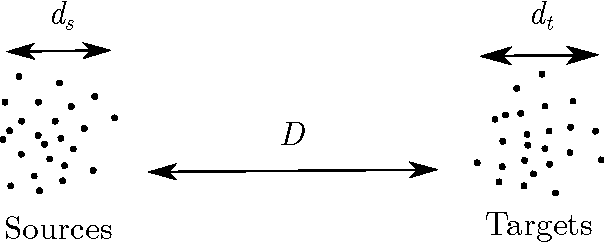
\includegraphics[width=0.5\textwidth]{introduction/degenerate_kernel.pdf}
    \caption{A set of source and target particle cluster, where the width of each cluster is significantly less than the distance separating them, $d_s, d_t \ll D$.}
    \label{fig:chpt:fmm:degenerate_kernel}
\end{figure}

Naively computed this requires $O(MN)$ operations. The \acrshort{fmm} relies on a \textit{degenerate} approximation of the interaction kernel when clusters of source and target particles are sufficiently separated, as sketched in Figure \ref{fig:chpt:fmm:degenerate_kernel}. Following the discussion in \cite{kailasa2024m2ltranslationoperatorskernel} the sum (\ref{eq:chpt:fmm:laplace_potential_sum}) can be written as,

\begin{equation}
    \phi(\Xbf_i) \approx \sum_{p=1}^P \sum_{j=1}^N A_p(\Xbf_i) B_p(\Ybf_j)q(\Ybf_j), \> \> i = 1,...,M
    \label{eq:chpt:introduction:sec:motivation:degenerate_kernel}
\end{equation}

where we call $P$ the expansion order, taken such that $P \ll N$, $P \ll M$. The functions $A_p$ and $B_p$ are defined by the approximation scheme used by a particular approach for the \acrshort{fmm}, in the original presentation the calculation,

\begin{equation}
    \hat{q}_p = \sum_{j=1}^N B_p(\Ybf_j)q(\Ybf_j)
\end{equation}

Corresponded to the coefficients of an order $P$ multipole expansion due to the source charges. Following which the potential is approximated by,

\begin{equation}
    \phi(\Xbf_i) \approx \sum_{p=1}^P A_p(\Xbf_i)\hat{q}_p, \> \> i = 1,...,M
\end{equation}

at the target particles. The approximation of the potential with this scheme can be seen to require $O(P(M+N))$ operations. The accuracy of this approximation scheme, and the error bounds provided by the \acrshort{fmm}, depends on the distance between the source and target clusters remaining large relative to their width. This condition is often referred to as an \textit{admissibility condition} in the \acrshort{fmm} literature. \acrshort{fmm}s therefore split the sum (\ref{eq:chpt:fmm:laplace_potential_sum}) into \textit{near} and \textit{far} components when considering arbitrary clusters of source and target particles,

\begin{equation}
    \phi(\Xbf_i) = \sum_{\Ybf_j \in \text{Near}(\Xbf_i)} K(\Xbf_i, \Ybf_j) q(\Ybf_j) +  \sum_{\Ybf_j \in \text{Far}(\Xbf_i)} K(\Xbf_i, \Ybf_j) q(\Ybf_j), \> \> i=1,..,M
\end{equation}

In cases where a source and target cluster can be considered \textit{admissable}, i.e. the source cluster is considered in the \textit{far field} of the target cluster such that each $\Ybf_j \in \text{Far}(\Xbf_j)$, we apply the approximation (\ref{eq:chpt:introduction:sec:motivation:degenerate_kernel}). However, when a source and target cluster are \textit{inadmissable}, such that the source cluster is considered in the \textit{near field} of a target cluster such that each $\Ybf_j \in \text{Near}(\Xbf_j)$ we are left to evaluate the sum directly via (\ref{eq:chpt:fmm:laplace_potential_sum}).

In order to achieve its $O(N)$ complexity the FMM is structured to reduce to a minimum the number of sums evaluated between inadmissable clusters. This is achieved with a hierarchical discretisation of the problem domain, often a \textit{quadtree} in two dimensions and correspondingly an \textit{octree} in three dimensions. These data structures are generated by creating a bounding box that covers the source and target particles, which without loss of generality may correspond to the same set. This box is then recursively sub-divided into \textit{child boxes} of equal size.

- Overview of FMM algorithm for non-Oscillatory kernels.

- A brief not on computing changes in the past decades, and which part of the algorithm are a little redundant.

- A reflection on the key hidden constants in complexity, and why this may no longer be the most significant factor in modern implementations.

- A note on FMM software that is available, its positives and negatives, and why this is a little different.

- Conclude with why this thesis exists, to tackle these problems.


\section{Kernel Independent Fast Multipole Methods}\label{chpt:fmm:sec:kifmm}

- Review of the KiFMM and variants. Black Box FMM, Analytical FMM, Data Driven Techniques.

- Motivation for use from a software engineering and computational performance perspective.

- Data flow during the KiFMM.

- Performance characteristics and features of the kiFMM.

- Reflection on the kiFMM and modern software and hardware

The decades since its original presentation have seen the \acrshort{fmm} extended with related ideas which principally differ in how they represent interactions between distant clusters of particles typically referred to as \textit{algebraic} FMMs.


- Black Box vs Analytical

\section{Oscillatory Fast Multipole Methods}

- helmholtz fmm

- high frequency helmholtz FMM, out of scope of the thesis but can mention that they exist. Especially in the context of kiFMM approaches, what is the key difference? When does it apply (the directional low rank condition), where is there an additional loop? Why might this result in greater complexity

\section{Related Ideas}

- H Matrix and H2 matrices, and wider setting of the FMM and related problems.

- Abduljabbar thesis contains a nice summary I can read.


\section{The Fast Multipole Method's Computational Structure}

- Parallelism levels in computing (ILP (Pipelining, Superscalar, Speculative execution), Data level (SIMD, GPU), Thread level TLP (multithreading, simultaneous multithreading and hyper threading), Process level (symettric and asymettrixc multitprocessing), task level, Distributed Parallelism e.g. MPI and MapReduce)

- Only some of these are relevant for scientific computing

- Examine FMM data flow and relate to levels of Parallelism and which will be taken advantage of by us, and which are yet to be examined.

- What is the trend in hardware and why is the FMM a good kernel for scaling in future computer systems?

- What are the principal difficulties we will encounter? Data organisation, and communication costs in a distributed setting.

- What about good FMM software? Specialised kernels and substructures are required to be generically interfaced.

- What parts of this are addressed by this thesis and where?


\section{Review of Software Approaches}

- What software exists, and which approaches do they use?

- What are they optimised for, and what kind of performance do they promise?

- What are the trade-offs of each software

- Hardware targetted by each available software, what's missing?

- What's available, and what are the shortcomings?

- And then

\section{Thesis Structure}\label{chpt:fmm:sec:layout}


In Chapter \ref{chpt:fmm} we perform a literature review of methods and software for modern \acrlong{fmm}s, with a specific focus on so called `kernel independent' or `black box' \acrshort{fmm}s in Sections ... and ... which are the focus of our implementation efforts. We review related ideas which share many features of the \acrshort{kifmm}s in Section ..., such as the $\mathcal{H}$ and $\mathcal{H}^2$ matrix approaches. We move on to a review of the \acrshort{kifmm}s computational structure in Section ..., where we provide estimates of the computational complexities of its operators, and identify the parallelism available in the algorithm with respect to that provided by modern hardware. We conclude with a review of past software efforts for \acrshort{fmm}s, and place our contribution within this context.


A major effort of this thesis was designing a \textit{platform} for \acrshort{kifmm}s. Whereby, one is free to experiment with the implementation of subcomponents in a highly modular way, while retaining performance and the use of the remainder of the library. Therefore a significant early investigation was into appropriate tooling environments for scientific software, first presented in \cite{kailasa2022pyexafmm}. We present this investigation in Chapter \ref{chpt:programming_for_science}, where we document our experience with Python as an alternative for achieving low-level performance as well as our chosen platform Rust, a relatively new language emerging as a contender for performant and productive research software.

Chapter \ref{chpt:field_translation} details a rigorous application of our framework, where we investigated optimisations for the crucial \acrshort{m2l} field translation, recently presented in \cite{kailasa2024m2ltranslationoperatorskernel}. We find non-intuitively that direct matrix compression techniques for admissable blocks can be highly competitive with state of the art optimal schemes based on \acrshort{ffts} for three dimensional problems described by the Laplace kernel.

Chapter \ref{chpt:software_design} describes in detail the engineering approach of our software, particularly the employment of Rust's trait system, as well as specific implementation details of the \acrshort{kifmm}s operators. In Chapter \ref{chpt:hpc} we discuss the design and implementation of our software framework for distributed memory systems, detailing communication reducing schemes for the communication of ghost information.

Chapter \ref{chpt:experiments} contains numerical experiments with our software in a single node (Section ...) as well as HPC (Section ...) setting, including a study of the applicability of our software to problems described by Helmholtz problems with low to moderate wavenumbers.


We conclude with a reflection on our results and suggestions for future investigations in Chapter \ref{chpt:conclusion}.



    \chapter{Modern Programming Environments for Science}\label{chpt:programming_for_science}
\thispagestyle{chaptertitle} % Force the fancy style on this page



\begin{center}
    \textit{The discussion in this chapter, including figures and diagrams, is adapted from the material first presented in \cite{kailasa2022pyexafmm}.}
\end{center}

\section{Requirements for Research Software}

- Requirements and constraints on research software development.

- As an example FMM softwares used in recent benchmark studies (ExaFMM variants, PVFMM) have been constructed during the course of doctoral or post-doctoral projects. This entails a significant `key man' risk, in which when the project owner completes their course of research the project enters a decay state and is no longer actively maintained and developed. New developers, unfamiliar with the code bases which can grow to thousands of lines of code, and often written without reference to standard software engineering paradigms for designing and managing large code bases (continuous integration, software diagrams, and simple decoupled interfaces) will find it challenging to build upon existing advances, and resort to developing new code-bases from scratch, rediscovering implementation details that are often critical in achieving practical performance.

- In seeking to avoid this cycle we envisioned a project built in Python, which maximises the maintainability of a project due to its simple syntax and language construction. New developers who, as a standard, are often educated in Python in the natural sciences and engineering, will hopefully be familiar with the language in order to gain productivity as fast as possible. However, as we demonstrated in our paper ... This itself imposes significant constraints on performance, which is balanced by the 'usability' of the language, making it just as challenging as developing a complex code in a compile language.

- Modern compiled languages offer tools that enable developer productivity. Examples include Go, Rust, ...

- The complexity of methods leads to complex code surface areas which are difficult to maintain especially in an academic setting with few resources for professional software engineering practice.

- The diversity of hardware and software backends leads to increasing difficulty for projects to experiment with and incorporate computational advances.

- Hardware and software complexity, and gap between a one-off coding project and extensible maintainable software tooling.

- Review developments in computer hardware and software that make this easier to be more productive, but also more challenging to wrap together over time.

- Emerging and future trends, exemplified by the step change in compiled langauges in the new generation and the interest in Rust and similar langauges. The mojo project and what this says about the future.


\section{Low Level or High Level? Balancing Programming Environments with Performance Requirements}

- Summary of Python paper results, in summary complex algorithms necessitate complex code in order to achieve performance - specifically the requirement for programmers to be in charge of memory and for hot sections manually vectorise etc. Writing everything in a high-level language obfuscates the application code from the sections critical to performance

- Review of why this was thought to be a good idea, and why it might be worth trying again in the future.

- What problems does this paper address, wrt to the literature?

- Brief review of motivation and reasoning behind Rust, and which features we take advantage of

- Review of data oriented design, how this can be enabled with traits.

% - Brief motivation behind fast particle solvers, and where they fit in the scientific landscape, why are they useful?

- Brief survey on other uses of FMM (Kalman filtering - covariance matrices), lead into application for integral equations which is our motivating application

- Give a sense of the scale of improvement that these methods provide for solving this class of problems - making integral equations practicable computational techniques is a big deal.

~ 1 page 
% \section{Pitfalls of Performant High Level Language Runtimes}\label{chpt:1:sec:1}

The evolution of computational science has been marked by the introduction and adoption of high-level interpreted languages that are designed to be user friendly, and cross platform. Starting with Matlab in the 1970s, followed by Python in the 1990s, and more recently Julia in the 2010s. High-level languages have significantly impacted scientific computing, offering efficient implementations of algorithms and introducing optimised data structures via projects such as NumPy and SciPy, as well as ergonomic cross platform build systems. While these languages facilitate easier experimentation, achieving peak performance often necessitates manual memory management or explicit instruction set level programming to ensure vectorisation on a given hardware target. A natural question for us when deciding on a programming environment for this project was whether advancements in high-level languages were sufficient for the implementation of `fast algorithms'. If they proved to be sufficient our software would be free of the so called `two language' problem, in which a user friendly interfaces in a high-level language provides a front-end for a compiled language implementation of more data-intensive operations. This problem plagues academic software development, as resulting software relies on a brittle low-level interface between the high-level front-end, and low-level back-ends for performance critical code sections.

Recent strategies to enhance the performance of high-level languages have involved refining compiler technology. These projects are advertised as tools that allow developers to use high-level languages for quick algorithm experimentation, while leaving it to the compiler to produce efficient machine code. Benchmarks are usually offered with respect certain numerical operations that can be vectorized, such as iteration over aligned data structures, with compilers taking care to unroll loops and apply inlining to inner function calls.

Noteworthy examples are the Numba project for Python and the Julia language. Both leverage the LLVM compiler infrastructure, which aims to standardize the back-end generation of machine code across various platforms. This approach, known as 'just in time' or JIT compilation, generates code at runtime from the types of a function's signature. Figure \ref{fig:chpt:1:sec:1:numba_runtime} provides a sketch of how Numba in particular generates machine code from high-level Python code. The LLVM compiler supports numerous hardware and software targets, including platforms like Intel and Arm, and provides multithreading through support for compiler extensions such as OpenMP. Additionally, these compilers offer native support for GPU code generation. An important difference between Numba and Julia is that Numba is simply a compiler built to optimise code written for the numerical types created using the NumPy library, and Julia is a fully fledged language. Numba contains implementations of algorithms a subset of the scientific Python ecosystem, specifically functionality from the NumPy project for array manipulation and linear algebra.

% Many `fast algorithms', such as the Fast Multipole Method (FMM), depend on hierarchical data structures. For instance a `quadtree', in two dimensions, and an `octree', in three dimensions. Here, each tree node points to either four or eight child nodes, respectively. A natural implementation makes use of pointers linking blocks of memory holding node data \cite{sundar2008bottom}. However, this method presents challenges in high-level programming environments that don't expose memory management to developers, and we are forced to linearise the data structure by making use of a linear blocks of memory to store node information, and vectors of index pointers to look up data.

As many performance benchmarks for these programming environments are typically provided for algorithms that rely on simpler data structures, we decided to test these high-level environments for more complex algorithms before making a choice about our programming environment for this project. We implemented a single node multi-threaded FMM using Python's Numba compiler, identifying two notable pitfalls with this approach, the full results of which were recently published in Computing in Science and Engineering \cite{kailasa2022pyexafmm}.

Firstly, JIT compilation of code imposes a significant runtime cost that is disruptive to development. Compiled functions are by default not cached between interpreter sessions in either Julia or Numba code. Our FMM code takes $15 \pm 1$s to compile when targeting a i7-9750H CPU with x86 architecture, where the benchmark is given with respect to seven runs. This is comparable to the runtime of the FMM software for a typical benchmark FMM problem \footnote{1e6 particles distributed randomly, using order $p=6$ expansions for a Laplace problem takes approximately 30s on this hardware using our software. See Chapter \ref{chpt:2:designing_software_for_fast_algorithms} for more details on the FMM and the significance of these terms.}. For smaller problem sizes, the compilation time dominates runtime. Ahead of time (AOT) compilation is partially supported in Numba, and can be used to build binaries for distribution to different hardware targets, e.g. x86 or ARM. However support for AOT compiled code is currently second class, the machine code created in this manner are usable only from the Python interpreter and not from within calls made from other Numba compiled functions, and it's currently staged for deprecation and replacement. We note that Julia does support AOT compilation via the PackageCompiler.jl module. This allows for different levels of AOT compilation, from creating a `sysimage' which amounts to a serialised file containing the compiled outputs of a Julia session, a relocatable `app' which includes an executable compiled to a specific hardware target alongside Julia itself, to creating a C library which can be precompiled for a specific hardware target such as x86. However, this requires relatively advanced software engineering skills, and raises the barrier to entry for high-performance computing with Julia.

Thus switching to such a programming environment requires developers to create a workflow that keeps interpreter sessions active for as long as possible in order to reduce the impact of long compilation times, or write build scripts for AOT compilation for a specific hardware target similar to compiled languages. As one of the key advantages of high-level languages is their developer friendliness and simple build systems this acts as an impediment.

Downstream users of software, who may also be using JIT compilers for their own code, are faced with significant compilation times, and potentially intricate build steps unless catered for by the original library's developers. This problem compounds in the case of distributed memory programs using MPI, as JIT compilation imposes runtime costs to the entire program. Unless a project has been distributed as a binary, by default MPI runs are not interactive, and therefore require a recompilation for each run. This isn't to say MPI programs written in Julia or Numba haven't been scaled to large HPC systems, however their usage does carry a cost in terms of developer workflow, and potentially program runtime, which can be significant if one is trying to reach the highest levels of performance.

Secondly, our experience in developing the FMM in Numba made clear how difficult it can be to anticipate the behaviour of Numba when considering how to optimise functions with different implementations of the same logic. Consider the code in Listing \ref{code:chpt:1:sec:1:numba_compiler_optimisations}, here we show three logically equivalent ways of performing two matrix-matrix products, and storing a column from the result in a dictionary. A dictionary is chosen for storage as this mirrors the data structure used in our FMM software for storing intermediate results. The runtimes of all three implementations are shown in Table \ref{table:chpt:1:sec:1:numba_compiler_optimisations} for different problem sizes. We choose this example because this operation of matrix-matrix multiplication is well supported by Numba, and data instantiation, whether from within or external to a Numba compiled function, should in principle make little difference as the Numba runtime simply dereferences pointers to heap allocated memory when entering a Numba compiled code segment. This example is designed to illustrate how arbitrary changes to writing style can impact the behavior of Numba code. The behavior is likely due to the initialisation of a dictionary from within a calling Numba function, rather than an external dictionary, and having to return this to the user. However, the optimisations taken by Numba are presented opaquely to a user and it's unclear why there are performance variations at all.

In developing our FMM code we faced significant challenges in tweaking our code and data structures to maximise the performance achieved from within Numba. From manually inlining subroutines as in Listing \ref{code:chpt:1:sec:1:numba_compiler_optimisations}, to testing where to allocate data. Our final code took a significant amount of time to develop, approximately six months, and was organised in a manner that optimised for performance rather than readability. Thus, despite being a \textit{compiler} for numerical Python, Numba behaved in practice more like a \textit{programming framework} which a developer had to adhere to strictly in order to achieve the highest-level of performance. The disadvantage of this is that the framework is both relatively restrictive, but also presented opaquely to a user.

Therefore, while being an amazing technology with great features, Numba was not decided to be a suitable choice for our programming environment. Its ability to target a diverse set of hardware targets from Python, leveraging the power of LLVM to write multithreaded, and autovectorised code, as well as writing CPU and GPU code from within Python, while allowing downstream projects to develop in a familiar language with a large open-source ecosystem and simple dependency management demonstrate the utility of this remarkable tool. However, the constraints of high level languages, specifically the inability to manage memory at a system level, as well as the development costs of JIT compilation, and Numba's framework-like behaviour demonstrate that while being useful, it is preferable to write our software platform using a systems-level language where high-performance can be assumed. Our criticisms of Numba also apply to Julia. However we note that Julia has certain advantages over Numba including its design and syntax focussed on mathematical computing, native support for multithreading, a richer type system and a large open-source community with a scientific computing focus.

System level languages have progressed commensurately to high-level languages over recent decades. Modern languages such as Go and Rust, offer runtimes with informative compilers, inbuilt documentation and testing facilities, as well as LLVM backends to support code generation across platforms, removing much of the complexity associated with building and distributing software written in C/C++. Rust in particular, uninhibited by a garbage collector as for Go, makes it easy to interoperate Rust code with libraries built in C/C++ via its foreign function interface, making it simple to leverage existing open-source scientific software.  We therefore conclude that the two language problem is minimised in comparison to the past, and modern system level programming languages potentially offer an effective solution for building academic software.

\begin{figure}[h]
    \centering
    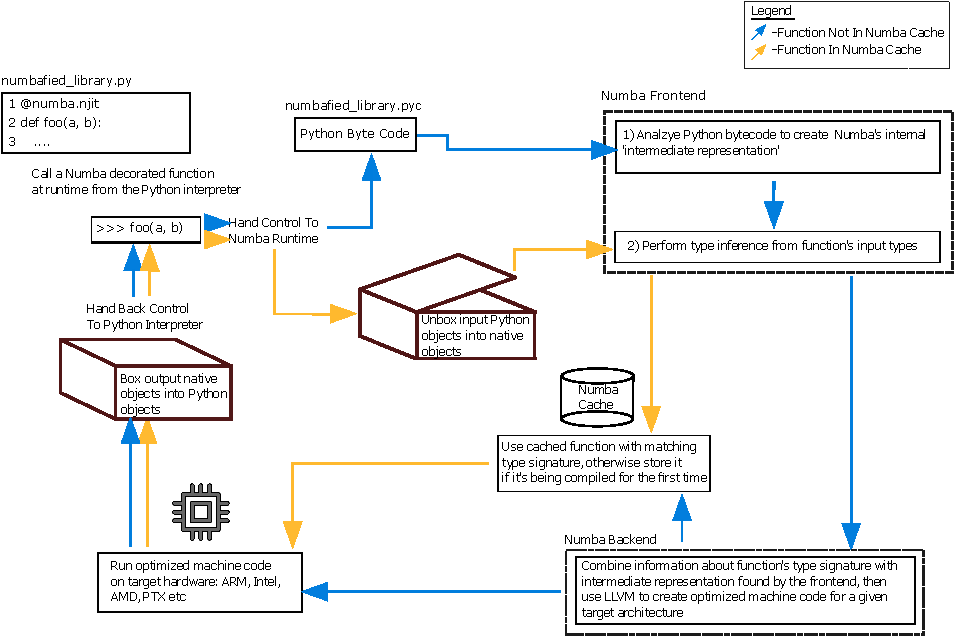
\includegraphics[width=\linewidth]{images/ch_1/numba.pdf}
    \caption{A visualisation of the Numba runtime system. A function decorated with `njit' acts as an instruction to the runtime to check a database for any Numba-compiled functions with a matching function signature, if this doesn't exist Numba generates a new compiled function and caches it using LLVM. Future calls of this function use this cached version in place of the Python interpreter. Code relies on Numba's runtime to correctly `box' and `unbox' native Python objects into data structures compatible with Numba code, which operates on a subset of numerical data structures created using the NumPy library. Figure adapted from \cite{kailasa2022pyexafmm}.}
    \label{fig:chpt:1:sec:1:numba_runtime}
\end{figure}


\pagebreak

% \begin{figure}[H]
\begin{lstlisting}[language=Python, caption={Three ways of writing a trivial algorithm in Numba, that performs some computation and saves the results to a dictionary. Adapted from Listing 2 in \cite{kailasa2022pyexafmm}},  label=code:chpt:1:sec:1:numba_compiler_optimisations]
import numpy as np
import numba
import numba.core
import numba.typed

# Initialise in the Python interpreter
data = numba.typed.Dict.empty(
    key_type=numba.core.types.unicode_type,
    value_type=numba.core.types.float64[:]
)

data['initial'] = np.ones(N)

# Subroutine 1
@numba.njit
def step_1(data):
    """
    Initialise a matrix and perform a matrix matrix product,
    storing a single column in the data dictionary.
    """
    a = np.random.rand(N, N)
    data['a'] = (a @ a)[0,:]


# Subroutine 2
@numba.njit
def step_2(data):
    """
    Initialise a matrix and perform a matrix matrix product,
    storing a single column in the data dictionary.
    """
    b = np.random.rand(N, N)
    data['b'] = (b @ b)[0,:]


@numba.njit
def algorithm_1(data):
    """
    First implementation.
    """
    step_1(data)
    step_2(data)


@numba.njit
def algorithm_2(data):
    """
    Second implementation.
    """
    # This time the storage dictionary is created within the
    # Numba function, so the types are inferred by the Numba
    # runtime, this also avoids a boxing cost to create a Numba
    # type from a Python one.
    data = dict()
    data['initial'] = np.ones(N)
    step_1(data)
    step_2(data)
    return data

@numba.njit
def algorithm_3(data):
    """
    Third implementation.
    """

    # This time, the subroutines are manually inlined
    # by the implementer, as well as the initialisation
    # of the results dictionary locally, as in algorithm_2.

    data = dict()
    data['initial'] = np.ones(N)

    def step_1(data):
        a = np.random.rand(N, N)
        data['a'] = (a @ a)[0,:]


    # Subroutine 2
    @numba.njit
    def step_2(data):
        b = np.random.rand(N, N)
        data['b'] = (b @ b)[0,:]

    step_1(data)
    step_2(data)
    return data
\end{lstlisting}
% \end{figure}
% \afterpage{\clearpage}


\begin{table}
    \centering
    \caption{Performance of different algorithms from Listing \ref{code:chpt:1:sec:1:numba_compiler_optimisations}, taken on an i7 CPU and averaged over seven runs for statistics.}
    \begin{tabular}{l l l}
        \toprule
        Algorithm & Matrix dimension & Time ($\mu s$) \\
        \midrule
        1 & \(\mathbb{R}^{1 \times 1}\) & 1.55 $\pm$ 0.01 \\
        1 & \(\mathbb{R}^{100 \times 100}\) & $304 \pm 3$\\
        1 & \(\mathbb{R}^{1000 \times 1000}\) & $29,100 \pm 234$ \\
        \midrule
        1 & \(\mathbb{R}^{1 \times 1}\) & $2.73 \pm 0.01$ \\
        1 & \(\mathbb{R}^{100 \times 100}\) & $312 \pm 3$ \\
        1 & \(\mathbb{R}^{1000 \times 1000}\) & $25,700 \pm 92$ \\
        \midrule
        1 & \(\mathbb{R}^{1 \times 1}\) & $2.71 \pm 0.01$ \\
        1 & \(\mathbb{R}^{100 \times 100}\) & $312 \pm 1$ \\
        1 & \(\mathbb{R}^{1000 \times 1000}\) & $25,700 \pm 140$ \\
        \bottomrule
    \end{tabular}
    \label{table:chpt:1:sec:1:numba_compiler_optimisations}
\end{table}

% \section{Introducing Rust for Scientific Software}\label{chpt:1:sec:2}

Rust is a modern system-level programming language, introduced by Mozilla in 2015 as a direct replacement for C/C++, and is bundled with features that favour safety for shared memory programming. Having identified it as a suitable candidate for our programming environment, we list a few of its key benefits in this section.

Fortran and C/C++ have have continued to dominate high-performance scientific computing applications, the main criticism of these languages for academic software is their relatively poor developer experience. C/C++ especially has significant flexibility in the compilers, documentation, build systems and package managers that developers can choose to work with, as well as support for multiple paradigms and a growing syntax. Rust stands in contrast to this with a single centrally supported runtime system, Cargo, with common standards for testing and documentation. Additionally, there is only a single Rust compiler, rustc. This inflexibility, in addition to a strongly preferred way of organising Rust code via its Traits system, makes Rust libraries significantly more uniform and readable than corresponding C++ code. Indeed installing a Rust library, or building a binary, is often as simple as running a single command from a terminal, or adding a single line to a TOML dependency file.

The lack of a uniform building and packaging standards in C/C++ means that some projects go as far as to implement a custom build system, such as the Boost library \cite{boostbuild2022github}. With the exception of Fortran, which has made recent strides to develop a standardised modern package manager and build system, inspired by Rust's Cargo \cite{fpm2022github}, C and C++ do not have a single officially supported package manager or build system. The resulting landscape is a multitude of package managers \cite{spack2022github, vcpkg2022github, conan2022github} and build systems \cite{meson2022github, bazel2022github, scons2022github} a few of which we have cited here, all of which replicate each others functionality, none of which are universally accepted or implemented across projects nor officially supported by the C++ software foundation. Figure (\ref{fig:chpt:1:sec:2:builds}) provides an overview of a few of the myriad approaches taken in other languages. To manage this complexity, builds are often defined using a metabuild system, most commonly CMake. CMake is a scripting language, and as a meta build system it takes a specification of local and third party dependencies and hardware targets, and generates Makefiles. CMake gives developers a great deal of flexibility, it is multi-platform, and language agnostic, however it is not straightforward to maintain projects as the number of dependencies grows. Indeed, there is a significant body of literature discussing best practices with CMake \cite{scott2018professional}. However, CMake is not responsible for downloading and installing third party packages or verifying their relative compatibility, implementing its best practices is again left to users. Cargo's relative simplicity mirrors the simple build systems of high-level languages such as Python or Julia, and removes one of the main causes of development pain when working with compiled languages, and makes it significantly easier for small teams to publish software that can be easily deployed by downstream users regardless of their system's architecture or operating system.

A unique feature of Rust is its approach to ensure safe shared memory programming, enforced by its compile time `borrow checker'. Every reference in Rust has an associated `lifetime' defined by its scope, and a singular `owner'. Which enforce the programming pattern of `resource allocation is initialisation' (RAII). The basic rule is that references are owned within a scope, and dropped when out of scope. The borrow checker enforces this at compile-time, in a multithreaded context this makes it impossible to have a compiled Rust binary that has dangling pointers or double-free errors. For mutable data, the borrow checker ensures that there is only a single mutable reference at any given time in the program's runtime, ensuring that there can never be a race condition in compiled Rust code. Identifying pointer-related bugs is one of the main challenges in multi-threaded programming, with safe `smart pointers' being optional in C++, implementing RAII is left to developers.

Rust is `multi-paradigm', supporting both object oriented, and functional styles of programming. Method calls are often chained, in a functional-like style, however users can still implement methods on structs as in other object oriented languages. The unique feature introduced by Rust is its Traits system, for specifying shared behaviour, that supersedes object-oriented design. Traits are a similar to C++ 20's interfaces, in that they provide a way to enforce behaviour, rather than embedding it into a type as with traditional inheritance. However unlike C++, Rust Traits allow you to write blanket implementations, and implement interfaces for types you didn't define in your own code making them significantly more powerful. This means that behaviour can be built `bottom up', rather than `top down' as with object orientation, making it much easier for readers to identify the expected behaviour of a given Rust type by simply reading which Traits it implements. In a scientific context we are usually concerned with the organisation, reading and writing of data, commonly adhering to a design philosophy known to as data-oriented design. Traits allow us to inject additional behaviour on types without having to worry about potentially complex inheritance hierarchies.

Rust's runtime includes a test runner, a documentation generator, and a code formatter. As with other Rust features, these are maintained in lock step with the language specification, and with reference to other Rust developments. This imposes universal constraints on all Rust projects, allowing for objectively defined `good' Rust code, rather than relying on various standards of best practices that vary between projects and organisations. Furthermore the Rust compiler is highly informative, providing hints to developers on best practices for their code, as well as potential sources of bugs or code rot, by notifying users of common anti-patterns or unused variables and functions.

Despite being a young language, Rust already supports a mature ecosystem of libraries for scientific computing with high-level multithreading support \cite{rayon2018github}, numerical data containers \cite{ndarray2022github}, and tools for generating interfaces to Python via its C ABI \cite{maturin2022github}. Many tools are yet to be ported into native Rust, however high quality bindings exist for core tools such as MPI \cite{rsmpi2018github}, BLAS and LAPACK \cite{blaslapackrust2022github}, with simplified build steps often requiring only a few extra lines in the dependency TOML file. The problem with interfacing with tools written in other languages is also present when building software in Rust, however Cargo offers tools to build software written in other languages and integrate it with Rust code via the `build.rs' package, which allows one to leverage existing build systems written for software written in foreign languages. This detracts from the benefits offered by Cargo as a unified package manager and build system, raising similar problems to those encountered when building software in other compiled languages. However, we observe that this remains a concern of the software's developer, who is responsible for providing build scripts for the operating systems and hardware platforms that they wish to support, and from a downstream user perspective their build process remains the same as with pure Rust packages, where the dependency is defined in their dependency TOML file. We also note that Rust is missing key tools for scientific computing, such as a code generation for GPUs, however with mounting interest in Rust from the scientific computing community this is an active area of development.


\begin{figure}
    \centerline{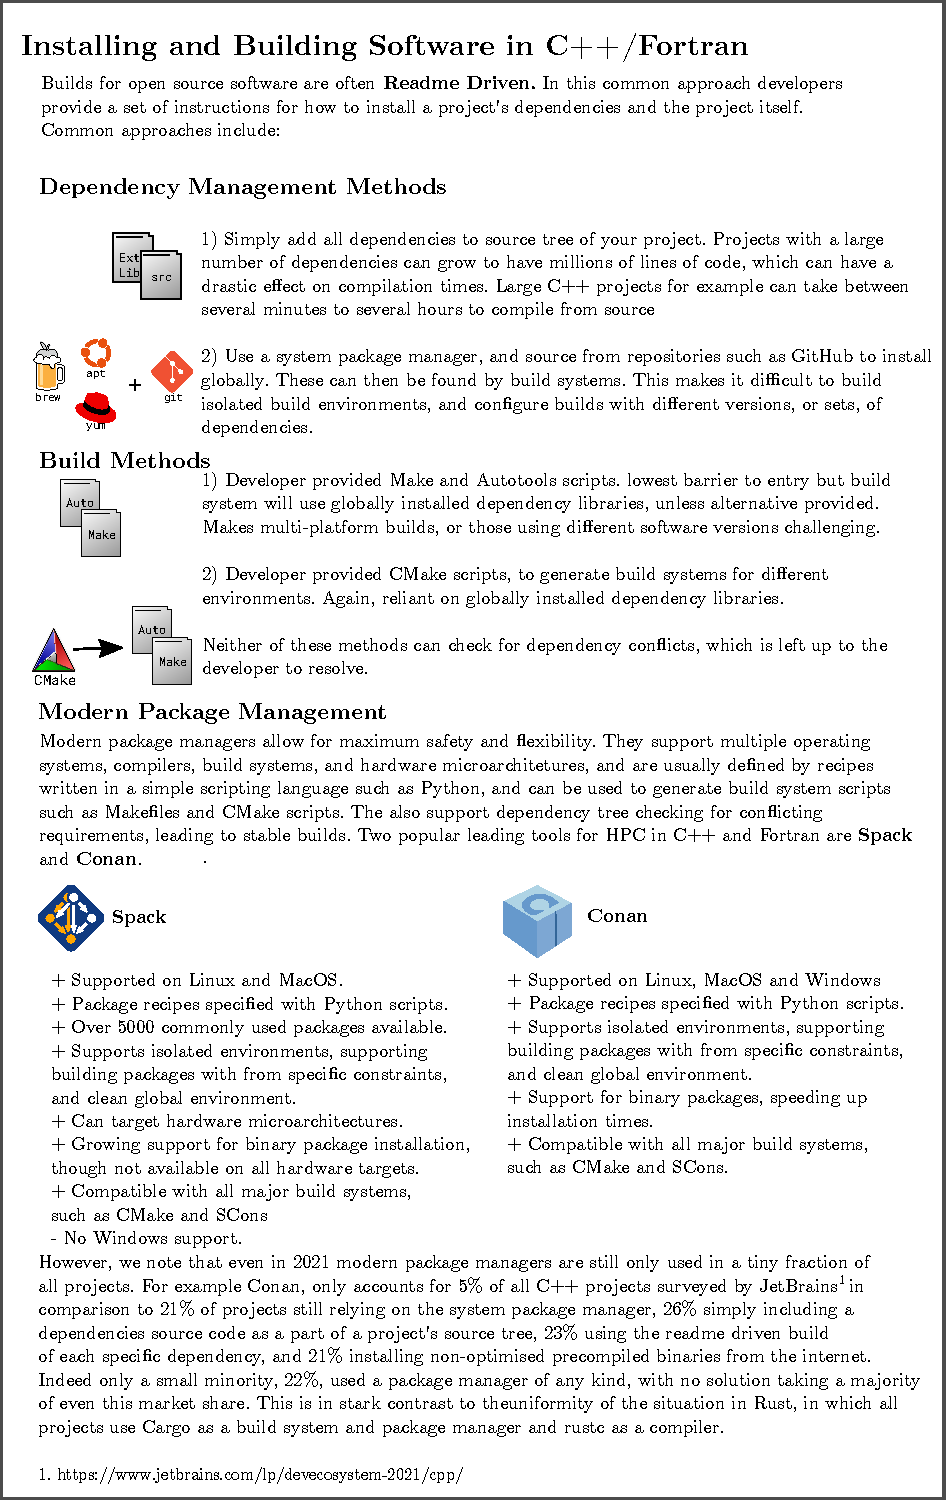
\includegraphics[width=0.95\linewidth]{ch_1/builds.pdf}}
    \caption{An overview of building software in other compiled languages.}
    \label{fig:chpt:1:sec:2:builds}
\end{figure}

% \section{Future Developments}\label{chpt:1:sec:3}

Despite the above criticisms, high-level languages as tools for high-performance scientific computing remain an intense area of research and development. 'Mojo' is a new programming language, along with a compiler. It's built as a superset of Python, specifically with the two-language problem in mind. Additionally, it attempts to address the 'three language problem', whereby languages also target exotic hardware such as GPUs and TPUs \cite{Lattner2023Mojo}.

Led by a team that includes the original developers of LLVM, Mojo aims to simplify the development of high-performance applications in a Python-like language, that acts as a superset of Python. Moreover, it seeks to make these applications deployable across most hardware and software targets, ensuring compatibility with Python's vast open-source libraries and straightforward build tools.

This is achieved by building on the MLIR compiler infrastructure. MLIR can be thought of as a generalisation of LLVM, catering to CPUs, GPUs, and novel ASICs for AI. The team chose to develop around Python to leverage its extensive existing user base in computational and data sciences.

Currently, Mojo remains a closed-source language and is actively being developed by its parent company, Modular. Thus, even though it appears promising, it's not yet in a state suitable for experimentation. Nevertheless, Mojo showcases the potential of a future programming environment that might definitively `solve' the problems developers face when selecting a programming environment for academic software.


    \chapter{High Performance Field Translations for the kiFMM}\label{chpt:field_translation}
\thispagestyle{chaptertitle} % Force the fancy style on this page

\begin{center}
    \textit{The discussion in this chapter, including figures and diagrams, is adapted from the material first presented in \cite{kailasa2024m2ltranslationoperatorskernel} }
\end{center}


\section{The Multipole to Local Translation (M2L)}\label{chpt:field_translation:sec:m2l}

- From chandrowlishwaram 2010 to now, the M2L has become the key bottleneck in terms of optimising kiFMM implementations. Cost of DRAM access hasn't scaled as quickly as available flops.

- Note here on the computational structure of the M2L problem. How it's poorly matched to modern CPU/GPU.

- We've already observed the M2L operator to be of convolution type, and therefore amenable to FFT acceleration if using regular grids like in the kiFMM.

- This has optimal complexity, but the low arithmetic intensity of the internal Hadamard product is difficult to optimise out.

- We postulate that direct matrix compression techniques, with specially designed hardware features that optimise for BLAS, as well as randomised methods for matrix compression - reducing pre-computation time, can result in highly competitive runtimes. Very high arithmetic intensity

- Introduce this subchapter

\subsection{Literature Review}

- use this section to introduce idea of transfer vectors, reflection and rotational symmetry

- Full literature review of past approaches

- Dense and Analytical approaches

- The historical push for this originally resulted in point and shoot/diagonal forms ('new' FMM paper)

- Where past efforts have been focussed, and why? (Original paper dismissed direct matrix compression)

- how this is achieved in practice (i.e. what computations are needed, not the implementation details)

- Explanation of the FFT method, and why it was able to achieve high performance.

- Why this may not be completely appropriate, low arithmetic intensity (maybe estimate?)

- How PVFMM makes it work, with very high arithmetic intensities, and special structure.

- Some criticism here of that approach.

- Require a special implementation for each architecture, intricate to maintain, requires passing mutable pointers over threads. Difficult to replicate, ours is the only re-implementation of this scheme in the open-source.

- Give the gist here, the actual details can be shoved in the appendix as it's not really a part of the discussion.

- Numerical compressoin of low rank blocks, approaches
- ie. how is SVD handled for aspect ratio
- randomised SVD
- estimating cutoff rank
- power iterations, and practical considerations
    - multithreading, where to use rSVD, limitation due to internal QR required, potentially alternative schemes - krylov-schur

- Alternative recompression scheme based on QR

\begin{flalign}
    A = BC^T, \text{ with } B \in \mathbb{R}^{m \times K}, C \in \mathbb{R}^{n \times K}
\end{flalign}

where $K > k$ target rank, but still much smaller than $m,n$.

\begin{enumerate}
    \item Compute Economic QR (cheaper than det SVD) $B = Q_BR_B$, $C = Q_C R_C$.
    \item  Compute truncated SVD $T_k(R_B, R_C^T) = \tilde{U}_k \Sigma_k \tilde{V}_k$
    \item Set $U_k = Q_B \tilde{U}_k$, $V_k = Q_C\tilde{V}_k$, return $T_k(A) := U_k \Sigma_k V_k^T$
\end{enumerate}

Complexity is $O((m+n)K^2)$, but smaller constant than SVD.


When $A$ does not have rank $k$ but can be well approximated by a rank - $k$ matrix, it is advisable to choose the oversampling parameter $p$ larger than 0 in the rSVD (alg 2 in Kressner review).  The following result shows that the resulting error will not be far away from the best approximation error $sigma\_k+1$ in expectation, with resepct to the the random matrix $\Omega$,

- Theorem, Let $k \geq 2$ and $p \geq 2$ be chosen such that $k+1 \leq \min\{m,n\}$. Then the rank-$k$ approximation $\tilde{A}$ satisfies

\begin{flalign}
    \mathbb{E}\|A-\tilde{A}\| \leq \left(2 + \frac{4\sqrt{(k+p)\min{\{m, n\}}}}{p-1}\right)\sigma_{k+1}
\end{flalign}

The bound improves significantly when performing a few steps of subspace iteration after Step 2 in Algorithm2, which requires a few additional block matrix-vector multiplications with AT and A. In practice, this may not be needed. As the following example shows, the observed approximation error is much better than predicted by Theorem above

Can here demonstrate compression of Laplace operator with different oversampling paremeters and observe how close erorr is to $\sigma_{k+1}$, use this to justify lack of power iterations.

- Need Singular value distributions for Helmholtz kernel to justify the parameters for compression, that investigation needs to be in this section. Similar to the Darve paper, i.e. to justify the approximate rank for the rSVD.

- Why might this be preferred, or advantageous, what are its constraints

- structure of modern CPU and GPU

- emerging CPU architectures with specialised units for matrix multiplication
    - examples of CPUs, apple M series, Qualcomm snapdragon

- implications for matmuls on GPU (low-precision)

- Using numerical compression schemes for low-rank blocks has a long history in the H matrix community
    - ACA, 'adaptive' expansion order schemes.
    - can be seen to correspond to 'variable expansion order FMM' schemes of the 90s/00s.

\subsection{A New Direct Compression Based Acceleration Scheme}

- Pioneering work by messner et. al. took these schemes and specifically focussed on computational aspects, the SVD is an expensive algorithm, worked on re-ordering the computation to reduce expense
    - we build on this
- Furthermore they worked on re-organising application to improve caching, and our approach extends this.


- Precomputations required for Laplace and Helmholtz, required storage.
- Why 'storage' is perhaps irrelevant - shallow trees, and anyways data movement rather than storage is critical.

- Approaches for BLAS based field translation in some more detail than in the paper.

- Essentially, we extend the idea of Messner et. al by completely unrolling the M2L loop via precomputatioan of critical metadata.

- Explanation of what metadata is required, what we mean by unrolling.

- Demonstrate how this is actually a general variant of what's been done in other approaches.

- This specification is very suggestive of an approach that relies on linear data structures and preserves cache-coherence.

- Suggests that a simple method using BLAS and multithreading can be highly effective, in contrast to the runtime systems experimented with in the past decades, simply because the cache structure of these computations is simple, and runtimes may destroy this.

- Algorithm itself, take from paper

- Caching experiment vs ScalFMM. Why software comparisons can be contrived, due to the vast differences in implementation details -e.g. kernel evaluations, but can directly compare the M2L runtimes alone for different expansion orders and tree levels.
    - cache destroyed by granular tasking approach

- The numerical results from the paper for Precomputations as well as M2L application cost. Need the same results for Helmholtz, but first need to find optimal parameters.

- Comment and discussion from the paper can be lifted here.

- Interesting point of comparison with ScalFMM to demonstrate the importance of caching to performance, noting that direct software comparisons are not entirely fair, but we are relying on same compiler version, threading model, and BLAS versions. The only difference being the organisation of the computation.

- Time just the M2L for ScalFMM, multithreading enabled, on threadripper. Single and double precision if possible, at different expansion orders, for increasing tree depth,

Kressner discussion on approaches for low rank matrix factorisations (non-hierarchical)

- Martin Stoll Krylov schur
- Levitt and Martinsson Linear Complexity Black Box Compression
- Halko, randomised linear algebra
- ACA
- SVD
- Other methods from paper.



\section{Leaf Level Operators (P2P, L2P, P2M)}

- NOTE this is work taken from the green-kernels library, implemented within our group for green kernel evaluation.
- 6k loc.
- specialised for a couple of instruction sets + generic autovectorised implementation.
- How do the SIMD implementations work? Newton steps + fast inverse square root.
- sleef for special functions

From FMM side
- how are we blocking targets over threads?
- what are the implications of ultrafast direct calculations on CPU, and potential for even faster on GPU (low-precision).
- i.e. majority of computation can be handled directly quite effectively. Minimise M2L, and makes direct matrix compression techniques more attractive. Could handle these rapidly on the CPU, and especially in H100-like systems with UMA, offload expensive direct computation to GPU.
- how could we translate our current codes to a GPU for P2P, what are the trade-offs? Would memory transfer mean that it's never worth it?

\section{Parent to Child Operators (M2M, L2L)}

- Formulation as BLAS3
    - specifically I want to show the exact way that this is done
    - i.e. using morton-like (at the level of a level) encoding to lookup siblings/sets of siblings at once and apply BLAS3.
    - block sizes determined heuristically for a given architecture, but could in principle be estimate from available L2/L3 cache sizes.
    - storage, i.e. relative between parent and child, especially note that extra required if different expansion order taken per level.

\section{Field Translation in a Distributed Setting}

- Communication intensive MPI FMM phases are related to ghost data communication for the M2L and P2P (All other operators are inherently local).

- Ibeid et. al. provide estimates of communication complexity based on halos of both of these operators

- From Ibeid, add a derivation.

- How are these achieved in practice? Global/Local split, introduced by Abduljabbar and Yokota.

- Suggestive of hierarchical communication pattern.

- However, this is perhaps over-complicated.

- Domains of each processor are known via all-reduce. Therefore a-priori know exactly where all elements of locally contained interaction lists lie at problem setup.

- Given massive core-count, and relatively small total node count on pre-exascale systems like Archer 2 which are likely to persist. Global/local split can be further simplified - just choose a number of nominated nodes (even just one) for the global tree computation. Instead of hierarchical exchange, calculate required data exchange as a precomputation step, and can then tune chunk-wise data exchange over all data using neighbourhood communicators. Much simpler to setup than multiple function calls at each level of the hierarchy, and allows for finer tuning of data exchange.

- Note, each AMD Epyc node on Archer 2 can easily handle problem sizes O(1e7) points in ~0.5s in double precision.



    \chapter{Software Design}\label{chpt:software_design}
\thispagestyle{chaptertitle} % Force the fancy style on this page


\section{Data Oriented Design with Rust Traits}

- Motivation, and review, DOD book.

- How do traits enable data oriented design.

- Overview of the design of the software.

- Diagram for principal traits and how they link together in the final software.

- Why is this good for the future? Well, it leaves open extension to other approaches for any individual subcomponent.

- An example of this is the genericity over data type, kernel implementation, and field translation method, with a space for the kind of tree data structure.

- Exactly how is decoupling achieved with trait interfaces?
    - decoupling of implementation from abstraction.

\section{FMM Software As A Framework}

- Want to encourage as much code re-use as possible.

- The re-implementation of critical subcomponents should be avoided. A step towards this is the development low-level C interfaces which enable the construction of higher level interfaces in compatible languages.

- We've made a start to this with a low-level interface to the principal API of the FMM software.

- We also want to be able to deploy on as wide a range of target hardware as possible, and leave open extension to future systems, enabled by design, referencing diagram.

- High level diagram of how software components fit together


- Code generation for multiple targets enabled by Rust's llvm based compiler.

- C ABI as a compatiblity layer to other projects, success with this in developing Python wrappers and integration with NGBEM

- Flexible backends enabled by RLST package for BLAS and Lapack.

\section{Case Study: A Trait Based M2L}

- How do metadata computations work for a configurable M2L implementation? What does the high-level framework expect of an M2L implementation?

- What does this look like in practice? Exactly what traits are there, how can re-implement them for an alternative M2L implementation?


In principal, how could one also implement a new FMM, a new tree or a new operator for e.g. GPU?

This is incredibly compelling for an FMM software, as it can serve as a testbed for extension and algorithmic experimentation as well as comparison. E.g. we could attempt to use our framework to directly compare analytical and kiFMM methods, re-using the same kernel/lapack/blas backends, tree data structure, the only difference would be the translation operator implementations allowing for a fair comparison.

\section{High Performance Trees}

- Exactly how are Morton encodings done, and what are the drawbacks and alternatives. Hilbert encodings, ORB. How much difference do any of these things make?

- Tree Construction approach and algorithms
    - Morton encoding via lookup tables
    - neighbour finding
    - interaction list construction (fast)

- What did we end up doing, and what is the justification for these being good enough.
    - weakly adaptive vs fully adaptive FMM.
    - why?


Important implementation details
    - construction of interaction lists, neighbour finding.
    - construction of Morton encodings.
    - rapid data access, lookup tables/index pointers
    - trade-offs of approach in shared and distributed memory
        - e.g. adaptive vs weakly adaptive trees.
        - problems with load balancing approach etc

- How am I storing key data? I'm not using a pure Z order in the data layout, I'm storing by level in Morton order for ease of lookup of contiguous sibling data

- How are multi/single node trees designed?

- basically, have a very shallow struct, with trait interfaces that define the trees/fmm trees. This means that the actual tree is incredibly abstract, and flexible. Being able to query it like a single node tree means that kernel code is largely unchanged for operators.


\section{FMM Metadata}

- Arguably the most important part of setting up the calculation to be fast is calculating metadata effectively, i.e. need to move as much of the work away from the runtime as possible.

- Most important pieces here are figuring out how the interaction lists correspond to runtime data structures in M2L.






    \chapter{The Kernel Independent Fast Multipole Method for Distributed Memory Systems}\label{chpt:distributed_fmm}
\thispagestyle{chaptertitle} % Force the fancy style on this page

- Focus is on the maximal reduction in communication.

- what communication can and cannot be avoided?

- How the local/global split in terms of tree gives rise to optimal communication scheme.

- What simplifying assumptions can we take for most pre-exascale systems?

- Avoid sorting of Morton keys/point data, the local/global split gives us a way to statically partition tree across available resources - simplifying assumption if work with ncpu = pow(8).
- Not restricted to this, but makes threading simpler for local FMMs.

- Optimal implementation of MPI primitives for common data sizes.

- What will probably not work approaching exascale?
- the gather operation over all processes required for multiple steps of this algorithm - ghost exchange, multipoles at local root on nominated processor. How can these problems be addressed? Do they even matter for the problem sizes we're concerned with?



    \chapter{Numerical Experiments}\label{chpt:experiments}
\thispagestyle{chaptertitle} % Force the fancy style on this page


\section{Single Node}\label{chpt:experiments:sec:single_node}

\subsection{Laplace}

\subsection{Helmholtz}


\section{Multi Node}


    \chapter{Conclusion}\label{chpt:conclusion}

In this subsidiary thesis we've presented progress on the development of a new software infrastructure for fast algorithms. We've documented recent outputs towards this goal including foundational software as well as a algorithmic techniques. The main outputs being an investigation into programming languages and environments most suitable for scientific computing, a parallel load balanced octree library designed for high-performance,  as well as a proxy-compression based fast direct solver for acoustic Helmholtz scattering problems.

The immediate next steps of this project will be to publish our recent software results on octrees in an appropriate scientific journal. We also intend to continue the developments on fast direct solvers for oscillatory problems, and extend the RS-S framework to electromagnetic scattering problems described by Maxwell's equations. This would constitute a first fast direct solver for electromagnetic scattering problems. In the medium term, we plan to complete the implementation of the parallel FMM software, and the apply this to large scale boundary integral equation problems. This would entail the completion of the majority of our fast solver infrastructure. The final stage of this project will be the extension of our infrastructure to a parallel fast direct solver, and the simulation of large scale electromagnetic scattering problems.

    \appendix
    
\chapter{Deriving Local Expansion Coefficents from Multipole Expansion in $\mathbb{R}^2$}\label{app:locals}
Working in the setting in which we derived the multipole expansion in equation (\ref{eq:ch_2:multipole_expansions}),

\begin{flalign}
    \phi(x) = \sum_{j \in I_s} K(x, y)q_j = \log(x-c_s)\hat{q}_0^s + \sum_{p=1}^\infty \frac{1}{(x-c_s)^p}\hat{q}_p^s
    \label{eq:app:multipole_expansion}
\end{flalign}

Deriving the local expansion centered around the origin, where the bounding box of the targets, $\Omega_t$, is well separated from the source box, $\Omega_s$,

\begin{flalign*}
    \phi(x) = \sum_{l=0}^\infty \hat{\phi}^t_l (x-c_t)^l
\end{flalign*}

from the multipole expansion relies on the following expressions,

\begin{flalign*}
\log((x-c_t)-c_s) &= \log(-c_s(1-\frac{x-c_t}{c_s})) \\
&= \log(-c_s)  - \sum_{l=1}^\infty \frac{1}{l} \left( \frac{x-c_t}{c_s} \right) ^l
\end{flalign*}

and,


\begin{flalign*}
    ((x-c_t)-c_s)^{-p} &= \left( \frac{-1}{c_s} \right)^p \left( \frac{1}{1-\frac{x-c_t}{c_s}} \right)^p \\
    &=  \left( \frac{-1}{c_s} \right)^p \sum_{l=0}^\infty \binom{l+p-1}{p-1} \left( \frac{x-c_t}{c_s} \right)^l
\end{flalign*}

Substituting these expressions into (\ref{eq:app:multipole_expansion}), translated to be centred on $\Omega_t$

\begin{flalign*}
    \phi(x) &= \log((x-c_t)-c_s)\hat{q}^s_0 + \sum_{p=1}^\infty \frac{1}{((x-c_t)-c_s)^p}\hat{q}_p^s \\
     &= \log(-c_s)\hat{q}^s_0 - \left( \sum_{l=1}^\infty \frac{1}{l} \left( \frac{x-c_t}{c_s} \right) ^l\right) \hat{q}^s_0 + \sum_{p=1}^\infty \left( \frac{-1}{c_s} \right)^p \sum_{l=0}^\infty \binom{l+p-1}{p-1} \left( \frac{x-c_t}{c_s} \right)^l \hat{q}^s_p
\end{flalign*}

Identifying the local expansion coefficients as,

\begin{flalign*}
    \hat{\phi}^t_0 = \hat{q}^s_0 \log(-c_s) + \sum_{p=1}^\infty \frac{\hat{q}^s_p}{c_s^p}(-1)^p
\end{flalign*}

and,

\begin{flalign*}
    \hat{\phi}_l^t = \frac{-\hat{q}_0^s}{l c_s^l} + \frac{1}{c_s^l}\sum_{p=1}^\infty \frac{\hat{q}_p^s}{c_s^p} \binom{l+p-1}{p-1} (-1)^p
\end{flalign*}


\chapter{Hyksort}\label{app:hyksort}
The parallel splitter selection and HykSort algorithms are provided below. In terms of complexity analysis, we adapt the analysis provided in section 3.4 of \cite{sundar2013hyksort}. The main costs of SampleSort is sorting the splitters and the MPI collectives for data reshuffling. This can lead to a load imbalance and network congestion, represented by a constant $c$ below,

\begin{flalign*}
    T_{ss} = t_c c \frac{N}{p} \log \frac{N}{p} + (t_s + t_w p) \log^2 p + t_w c \frac{N}{p}
\end{flalign*}

Where $t_c$ is the intranode memory slowness (1/RAM bandwidth), $t_s$ interconnect latency, $t_w$ is the interconnect slowness (1/bandwidth), $p$ is the number of MPI tasks in $comm$, and $N$ is the total number of keys in an input array $A$, of length $N$.

The parallel splitter selection algorithm for determining $k$ splitters uses MPI collectives, \texttt{All\_Gather}() and \texttt{All\_Reduce}(). The main cost is in determining the local ranks of the samples using a binary search. The number of iterations $\eta$ depends on the input distribution, the required tolerance $N_\epsilon/N$ and the parameter $\beta$. The expected value of $\eta$ varies as $\log(\epsilon)/\log(\beta)$ and $\beta$ is chosen experimentally to minimise the running time, leading to a complexity of,

\begin{flalign*}
    T_{ps} = \eta t_c \beta k \log \frac{N}{p} + \eta (t_s + t_w \beta k) \log p
\end{flalign*}

HykSort relies on a specialised \texttt{All\_to\_all\_kway}() collective, we defer to the original paper for details. It uses only point to point communications with staged message sends and receives, allowing HykSort to minimise network congestion. It has $\log p / \log k$ stages with $O(N/p)$ data transfer and $k$ messages for each task in every stage. This leads to a complexity of,

\begin{flalign*}
    T_{a2a} = \left( t_s k + t_w \frac{N}{p} \right) \frac{\log p}{\log k}
\end{flalign*}

Finally, HykSort has the same communication pattern as \texttt{All\_to\_all\_kway}(). In addition it relies on the parallel splitter selection algorithm to determine splitters. The main computational cost is the initial local sort, and merging $k$ arrays during each iteration.

\begin{flalign}
    T_{Hk} = t_c \frac{N}{p} \log \frac{N}{p} + \left( t_c \frac{N}{p} + T_{ps}\right) \frac{\log p}{\log k} + T_{a2a}
\end{flalign}

Unlike SampleSort, the complexity of HykSort doesn't involve any $O(p)$ terms. This is the term that can lead to network congestion for higher core counts.

\begin{algorithm}
    \caption{\textbf{Parallel Select}}
    \begin{algorithmic}
        \STATE \textbf{Input:} $A_r$ - array to be sorted (local to each process), $n$ - number of elements in $A_r$, $N$ - total number of elements, $R[0,....,k-1]$ - expected global ranks, $N_\epsilon$ - global rank tolerance, $\beta \in [20, 40]$,

        \STATE \textbf{Output:} $S \subset A$ - global splitters, where $A$ is the global array to be sorted, with approximate global ranks $R[0,...,k-1]$

        \STATE $R^{\text{start}} \gets [0,...,0]$ - Start range of sampling splitters
        \STATE $R^{\text{end}} \gets [n,...,n]$ - End range of sampling splitters
        \STATE $n_s \gets [\beta/p,...,\beta/p]$ - Number of local samples, each splitters
        \STATE $N_{\text{err}} \gets N_\epsilon + 1$

        \WHILE{$N_{\text{err}} > N_\epsilon$}
            \STATE $Q' \gets A_r[\texttt{rand}(n_s, (R^{\text{start}}, R^{\text{end}}))]$
            \STATE $Q \gets$ \texttt{Sort}(\texttt{All\_Gather}($\hat{Q}'$))
            \STATE $R^{loc} \gets \texttt{Rank}(Q, A_r)$
            \STATE $R^{glb} \gets \texttt{All\_Reduce}(R^{loc})$
            \STATE $ I[i] \gets \text{argmin}_j | R^{glb} - R[I] | $
            \STATE $N_{err} \gets \max |R^{glb} - R{I}|$
            \STATE $R^{\text{start}} \gets R^{loc}[I-1]$
            \STATE $R^{\text{end}}  \gets R^{loc}[I+1]$
            \STATE $n_s \gets \beta \frac{R^{\text{end}}-R^{\text{start}}}{R^{glb}[I+1]-R^{glb}[I-1]}$
        \ENDWHILE
        \STATE \textbf{return }$S \gets Q[I]$
    \end{algorithmic}
\end{algorithm}

\begin{algorithm}
    \caption{\textbf{HykSort}}
    \begin{algorithmic}
        \STATE \textbf{Input:} $A_r$ - array to be sorted (local to each process), $comm$ - MPI communicator, $p$ - number of processes, $p_r$ - rank of current task in $comm$
        \STATE \textbf{Output:} globally sorted array $B$.
        \WHILE{$p > 1$, Iters: $O(\log p/\log k)$}
            \STATE $N \gets \texttt{MPI\_AllReduce}(|B|, comm)$
            \STATE $s \gets \texttt{ParallelSelect}(B, \{i N/k ; i=1,...,k-1 \})$
            \STATE $d_{i+1} \gets \texttt{Rank}(s_i, B), \> \forall i$
            \STATE $[d_0, d_k] \gets [0, n]$
            \STATE $color \gets \lfloor k p_r/p \rfloor$
            \PARFOR{ $i \in 0,...,k-1$}
                \STATE $p_{recv} \gets m((color-i)\text{mod}k)+(p_r \text{mod}m)$
                \STATE $R_i \gets \texttt{MPI\_Irecv}(p_{recv}, comm)$
            \ENDPARFOR

            \FOR{$i \in 0,...,k-1$}
                \STATE $p_{recv} \gets m((color-i)\text{mod}k)+p_r \text{mod}m$
                \STATE $p_{send} \gets m((color+i)\text{mod}k)+p_r \text{mod}m$
                \STATE $j \gets 2$
                \WHILE{$i > 0$ and $i \text{mod}j = 0$}
                    \STATE $R_{i-j} \gets \texttt{merge}(R_{i-j}, R_{i-j/2})$
                    \STATE $j \gets 2j$
                \ENDWHILE
                \STATE \texttt{MPI\_WaitRecv}($p_{recv}$)
            \ENDFOR
            \STATE \texttt{MPI\_WaitAll}()
            \STATE $B \gets \texttt{merge}(R_0, R_{k/2})$
            \STATE $comm \gets \texttt{MPI\_Comm\_splitt}($color, comm$)$
            \STATE $p_r \gets \texttt{MPI\_Comm\_rank}(comm)$
        \ENDWHILE
        \STATE \textbf{return } $B$
    \end{algorithmic}
\end{algorithm}

\chapter{Adaptive Fast Multipole Method Algorithm}\label{app:adaptive_fmm}
FMM literature distinguishes between types of relationships  between neighbouring nodes with the concept of \textit{interaction lists}. There are four such lists for a given node $B$, called $V$, $U$, $W$ and $X$. For a leaf node $B$, the $U$ list contains $B$ itself and leaf nodes adjacent to $B$. and the $W$ list consists of the descendants of $B$'s neighbours whose parents are adjacent to $B$. For non-leaf nodes, the $V$ list is the set of children of the neighbours of the parent of $B$ which are not adjacent to $B$, and the $X$ list consists of all nodes $A$ such that $B$ is in their $W$ lists. The non-adaptive algorithm is similar, however the $W$ and $X$ lists are empty

\begin{algorithm}
    \caption{\textbf{Adaptive Fast Multipole Method}.}
    \label{alg:fmm}
    \begin{algorithmic}

        \STATE $N$ is the total number of points
        \STATE $s$ is the maximum number of points in a leaf node.

        \STATE
        \STATE \textbf{Step 1: Tree construction}

        \FOR{each node $B$ in \textit{preorder} traversal of tree, i.e. the nodes are traversed bottom-up, level-by-level, beginning with the finest nodes.}
            \STATE subdivide $B$ if it contains more than $s$ points.
        \ENDFOR
        \FOR{each node $B$ in \textit{preorder} traversal of tree}
            \STATE construct \textit{interaction lists}, $U$, $V$, $X$, $W$
        \ENDFOR

        \STATE
        \STATE \textbf{Step 2: Upward Pass}
        \FOR{each leaf node $B$ in \textit{postorder} traversal of the tree, i.e. the nodes are traversed top-down, level-by-level, beginning with the coarsest nodes.}
        \STATE \textbf{P2M}: compute multipole expansion for the particles they contain.
        \ENDFOR
        \FOR{each non leaf node $B$ in \textit{postorder} traversal of the tree}
        \STATE \textbf{M2M}: form a multipole expansion by translating the expansion centre of its children to its centre and summing their multipole expansion coefficients.
        \ENDFOR

        \STATE
        \STATE \textbf{Step 3: Downward Pass}
        \FOR{each non-root node $B$ in \textit{preorder} traversal of the tree}
        \STATE \textbf{M2L}: translate multipole expansions of nodes in $B$'s $V$ list to a local expansion at $B$.
        \STATE \textbf{P2L}: translate the charges of particles in $B$'s $X$ to the local expansion at $B$.
        \STATE \textbf{L2L}: translate $B$'s local expansion to its children by translating its expansion centre to the centre of its children, and assigning the same coefficients.
        \ENDFOR

        \FOR{each leaf node $B$ in \textit{preorder} traversal of the tree}
        \STATE \textbf{P2P}: directly compute the local interactions using the kernel between the particles in $B$ and its $U$ list.
        \STATE \textbf{L2P}: translate local expansions for nodes in $B$'s $W$ list to the particles in $B$.
        \STATE \textbf{M2P}: translate the multipole expansions for nodes in $B$'s $W$ list to the particles in $B$.
        \ENDFOR
    \end{algorithmic}
    \end{algorithm}


    % \printglossary
    \printbibliography[heading=bibintoc]

\end{document}